%---------------------------------------------------------------------------
% PRIMEIRA SEÇÃO
\section{Introdução}

% SLIDE 1 - INTRODUÇÃO    
\begin{frame}
    \frametitle{Introdução}
    \framesubtitle{Visão Geral}
    \center

        TEXTO
        
\end{frame}


% SLIDE 2 - INTRODUÇÃO
\begin{frame}
    \frametitle{Introdução}
    \framesubtitle{Objetivos}
    \begin{itemize}
        
        \item Objetivo Geral:
        \begin{itemize}
        
            \item OBJETIVO GERAL

        \end{itemize}
        
        \item Objetivos Específicos:
        \begin{itemize}

            \item OBJETIVO ESPECÍFICO 1
            \item OBJETIVO ESPECÍFICO 2
            \item OBJETIVO ESPECÍFICO 3

        \end{itemize}
        
    \end{itemize}
\end{frame}

%---------------------------------------------------------------------------
% SEGUNDA SEÇÃO - FUNDAMENTAÇÃO TEÓRICA
\section{Fundamentação Teórica}

% SLIDE 3 - FUNDAMENTAÇÃO TEÓRICA
\begin{frame}
    \frametitle{Fundamentação Teórica}
    \framesubtitle{Tópico 1}
    
    De acordo com \citeonline{book}, (...) a Tabela \ref{table:1} 
    mostra...
    
    \begin{table}[h!]
        \centering
        \caption{Tabela.}
        \label{table:1}
        
            \begin{tabular}[]{cc}
                
                \hline
                Descrição 1 &  Descrição 2 \\
                \hline
                \hline
                Valor 1 $\pm$ desvio-padrão & $ 1000 \pm 2 $ \\
                Valor 2 $\pm$ desvio-padrão & $ 10000 \pm 20 $\\
                Valor 3 $\pm$ desvio-padrão & $ 100 \pm 0,2 $ \\ [1ex]
                \hline
            
            \end{tabular}
    
    \end{table}
    


\end{frame}

%---------------------------------------------------------------------------
% TERCEIRA SEÇÃO - METODOLOGIA
\section{Metodologia}

% SLIDE 4 - METODOLOGIA
\begin{frame}
    \frametitle{Metodologia}
    \framesubtitle{Tópico 1}
    
    A Figura \ref{fig:1} mostra...

    \begin{figure}
        
        \centering
        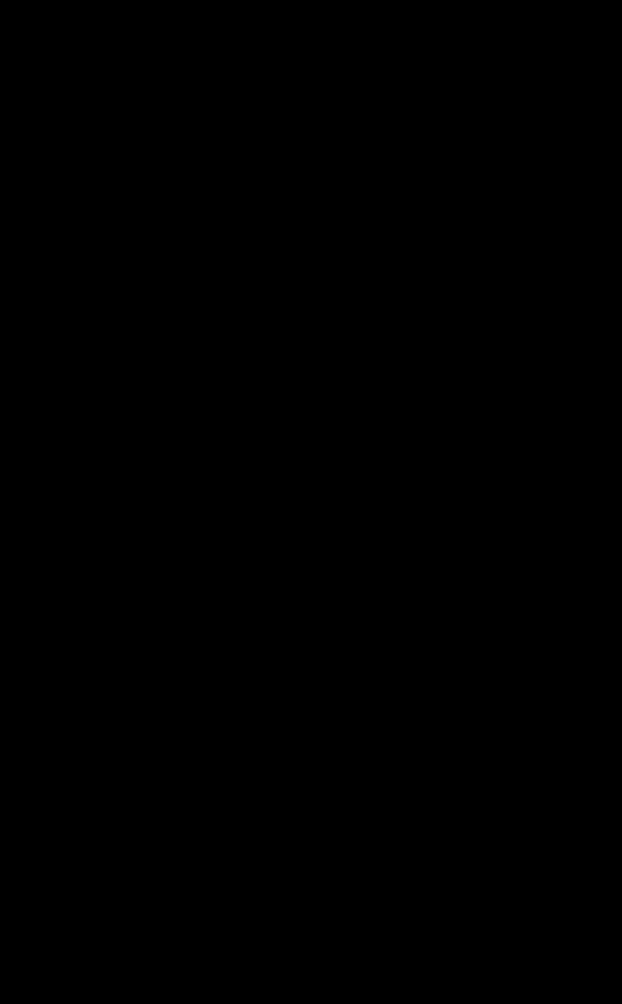
\includegraphics[width=0.2\linewidth]{example_image}
        \caption{Figura \cite{article}.}
        \label{fig:1}
        
     \end{figure}

\end{frame}

%---------------------------------------------------------------------------
% QUARTA SEÇÃO - RESULTADOS
\section{Resultados}

% SLIDE 5 - RESULTADOS
\begin{frame}
    \frametitle{Resultados}
    \framesubtitle{Tópico 1}
    
    \begin{columns}
        
        \begin{column}{0.5\textwidth}
            
            \begin{itemize}
                
                \item RESULTADO 1 (Figura \ref{fig:2});
                \item RESULTADO 2;
                \item RESULTADO 3;
                \item RESULTADO 4.
                
            \end{itemize}
        
        \end{column}
        
        \begin{column}{0.5\textwidth}
            
            \begin{figure}
        
                \centering
                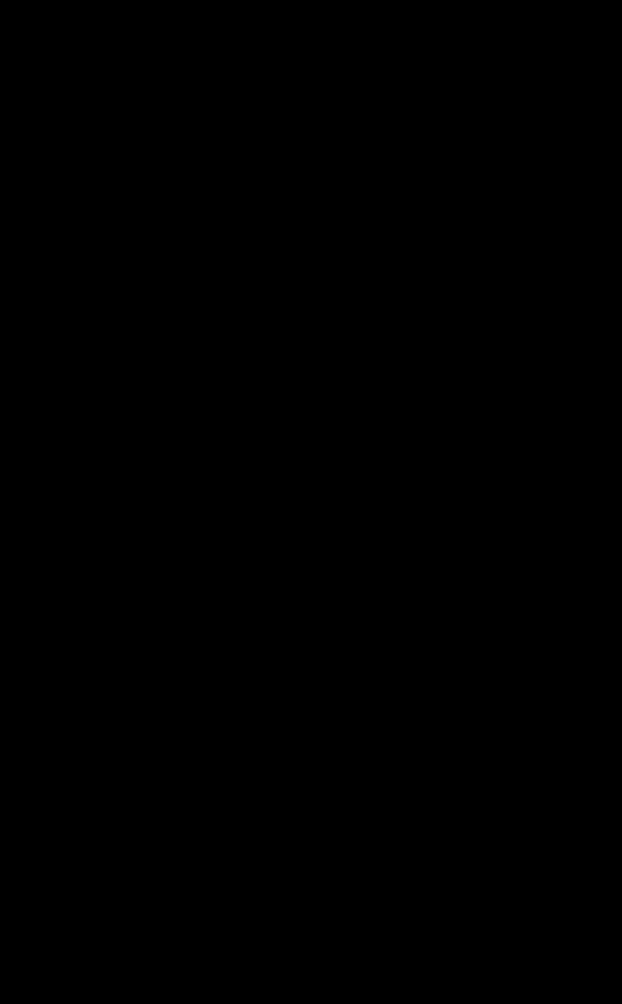
\includegraphics[width=0.5\linewidth]{example_image}
                \caption{Outra figura.}
                \label{fig:2}
        
            \end{figure}
        
        \end{column}
    
    \end{columns}
    
\end{frame}


%---------------------------------------------------------------------------
% QUINTA SEÇÃO - CONSIDERAÇÕES FINAIS
\section{Considerações Finais}

% SLIDE 6 - CONSIDERAÇÕES FINAIS
\begin{frame}
    \frametitle{Considerações Finais}
    %\framesubtitle{topico}
    \center

    CONSIDERAÇÕES FINAIS

\end{frame}
    
%---------------------------------------------------------------------------
